\documentclass{standalone}
\usepackage{tikz}
\usepackage{circuitikz}

\begin{document}
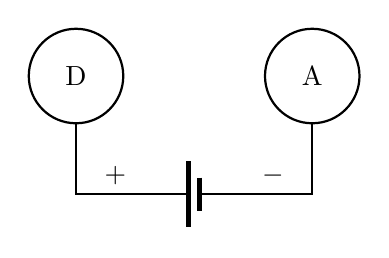
\begin{tikzpicture}[
    atom/.style={circle, draw=black, minimum size=1.2cm, thick}
]

  % Define variables for better adjustability
  \def\atomSep{3}         % Separation between atoms (horizontal distance)
  \def\rowSep{1.5}        % Base vertical spacing unit
  \def\batteryWidth{2}    % Width of the battery

  % Place the atoms (D for donor, A for acceptor)
  \node[atom] (D) at (0,0) {D};
  \node[atom] (A) at (\atomSep,0) {A};

  % Battery placement
  \coordinate (BatLeft) at  (\atomSep/2 - \batteryWidth/2, -\rowSep);
  \coordinate (BatRight) at (\atomSep/2 + \batteryWidth/2, -\rowSep);

  % Draw the battery
  \draw[thick] (BatLeft) to[battery1, name=Bat] (BatRight);

  % Add + and - labels above battery terminals
  \node[above] at (BatLeft)  {$+$};
  \node[above] at (BatRight) {$-$};

  % Connect atoms to battery terminals
  \draw[thick] (D) |- (BatLeft);
  \draw[thick] (A) |- (BatRight);

\end{tikzpicture}
\end{document}

